\documentclass[fleqn,reqno,10pt]{article}
\usepackage{amsmath}
\usepackage{amsfonts}
\usepackage{amsthm}
\usepackage{amssymb}
\usepackage{mathrsfs}
\usepackage{nicefrac}
%\usepackage{stmaryrd}
%\usepackage{multicol}
\usepackage{graphicx}
\usepackage{color}
\usepackage{booktabs}
\usepackage{pgfplots}
\usepackage{subcaption}

\usepackage{blkarray}
\usepackage{xspace}

\usepackage{tgtermes}
\renewcommand{\baselinestretch}{1.2}

\newcommand{\mylang}[1]{\ensuremath{L_{\text{#1}}}\xspace} %meaningful states
\newcommand{\mystate}[1]{\ensuremath{\state_{\text{#1}}}\xspace} %meaningful states
\newcommand{\mymessg}[1]{\ensuremath{\messg_{\text{#1}}}\xspace} %meaningful messages
\newcommand{\messg}{\ensuremath{m}\xspace}		% single messages
\newcommand{\state}{\ensuremath{s}\xspace}		% single states

\newcommand{\Lbound}{\mylang{bound}}
\newcommand{\Llack}{\mylang{lack}}
\newcommand{\ssome}{\mystate{\ensuremath{\exists\neg\forall}}}
\newcommand{\sall}{\mystate{\ensuremath{\forall}}}
\newcommand{\snone}{\mystate{\ensuremath{\emptyset}}}
\newcommand{\msome}{\mymessg{some}}
\newcommand{\mall}{\mymessg{all}}


\definecolor{mygray}{cmyk}{0.35,0.35,0.35,0.35}
\newcommand{\mygray}[1]{{\textcolor{mygray}{#1}}}


\title{Notes 2.0 on presentation of model for co-evolution}
\author{Thomas Brochhagen}
\date{}

\begin{document}
\maketitle

\subsection*{Motivation}

We would like to present our model in a cleaner and more intuitive way. As suggested by Michael, one way to do so is to focus first on a reduced type space to illustrate how the model works. As a reminder:

\begin{align*}
  \Lbound & = \begin{blockarray}{lcc}
    & \mygray{\msome} & \mygray{\mall} \\
    \begin{block}{l[cc]}
      \mygray{\ssome} & 1 & 0 \\
      \mygray{\sall}  & 0 & 1 \\
    \end{block}
  \end{blockarray} &
  \Llack & = \begin{blockarray}{lcc}
    & \mygray{\msome} & \mygray{\mall} \\
    \begin{block}{l[cc]}
      \mygray{\ssome} & 1 & 0 \\
      \mygray{\sall}  & 1 & 1 \\
    \end{block}
  \end{blockarray}
\end{align*}

These two lexica are paired with either level-$0$ {\em literal} behavior, or level-$1$ {\em pragmatic} behavior. Learnability-wise, if there is a bias for simpler semantics (no-upper bound), then the two types with $\Llack$ are favored {\em a priori}. Furthermore, both $\Lbound$ users are indiscernible when it comes to learning; they only differ in their receiver behavior. Utility-wise, literal $\Lbound$ fares slightly better than pragmatic $\Lbound$. If $\lambda$ is sufficiently high, then the difference between pragmatic $\Llack$ and both $\Lbound$ types is almost negligible. We want to visualize how (co-)evolution plays out by comparing four populations of two types each, where each pair of types differs only in (i) signaling behavior, or (ii) lexica:

\begin{enumerate}
  \item literal $\Lbound$ vs. literal $\Llack$;
  \item pragmatic $\Lbound$ vs. pragmatic $\Llack$;
  \item literal $\Lbound$ vs. pragmatic $\Lbound$;
  \item literal $\Llack$ vs. pragmatic $\Llack$.
\end{enumerate}

The other relevant parameters of the model are: soft-max parameter $\lambda$, posterior parameter $l$, sequence length $k$, and bias parameter $c$ (detailed below).

\subsection*{Learning bias}
In the paper, the learners' inductive bias is a function of the complexity of the formulae that types lexicalize. Introducing our measure and applying it only to this small type space is probably not the way to go. For illustratory purposes, we may instead assume that there's an abstract parameter (which we later make concrete using our measure) $c \geq 1$ that regulates how strongly $\Llack$ is preferred over $\Lbound$. In what follows, I assumed this to be $P(L_i) \propto c$ if $L_i$ is $\Llack$ and otherwise $1$. For instance, if we have  a type space with $\tau_i$ as literal $\Lbound$ and $\tau_j$ as pragmatic $\Llack$, then $P(\tau_i) \approx .33$ for $c = 2$. This is just for illustration, of course. We can change this at will. As far as I can see, the reduced type spaced behaves in a very predictable manner.% I set $c = 2$ for all the plots below.

\subsection*{General remarks 2.0}
There are three remarks to be made about this update.

First, the phase plots are a lot cleaner and all show stationary points. These were either calculated, or estimated as being in the middle of two points that changed in opposite directions. As before, the RD competition between literal and pragmatic $\Lbound$ is messy because there are many points for which $RD(x) = x$. On this front, I just changed white circles with black edges to red circles without edges for better visibility when many circles overlap.  

Second, when it comes to the direct competition of only two types on a line (phase plots), M and RMD still produce pretty similar outcomes. I tested a range of learning bias values and larger $k$ but there's not much change. This is not really troublesome (it being a consequence of there only being two types in a population), but I think this may disqualify the phase plots as candidates for a good illustration of the model's dynamics. 

Third, I tried my hand at the 2D quiver plots with all types, not only at the edges but also at the center of the unit square. As Michael suggested, $(x,y)$-pairs in the square give the following proportions of types:
\begin{itemize} 
  \item $lit. \; \Lbound$: $(1-x) * (1-y)$ 
  \item $lit. \; \Llack$: $(1-x) * y$
  \item $prag.\; \Lbound$: $x * (1-y)$
  \item $prag.\; \Llack$: $x * y$
\end{itemize}

Overall, I think these plots look good. Important, to me, is that (i) M and RMD are clearly distinguishable and that (ii) it's clear that RD with lowish $\lambda$ leads to $\Lbound$. Another plus is that it's easy to explain how this plot came about. On the negative side, I'm still a bit unhappy about having to assume that prag. and $\Llack$ are independent, but this is clearly better than just plotting the edges. The one important I am missing from these plots is clear movement on the lower edge, from $(1,0)$ to $(0,0)$, which would indicate movement from prag. $\Lbound$ to lit. $\Lbound$,  at least for RD-only. This would help us in driving the message home that pragmatic recruitment is not functionally advantageous for all types. I think the problem right now is that movement on this edge progresses in very small steps (if at all; cf. phase plots). These small steps disappear once we scale them with the bigger change that happens elsewhere in the square. Reinterpreting $(x,y)$ would not help on the edge itself, but maybe taking average trajectories would at least make points close to the edge move toward lit. $\Llack$ rather than toward its pragmatic counterpart. 

\subsection*{Phase portraits}
\begin{figure}
\centering
\begin{subfigure}{.6\textwidth}
  \centering
  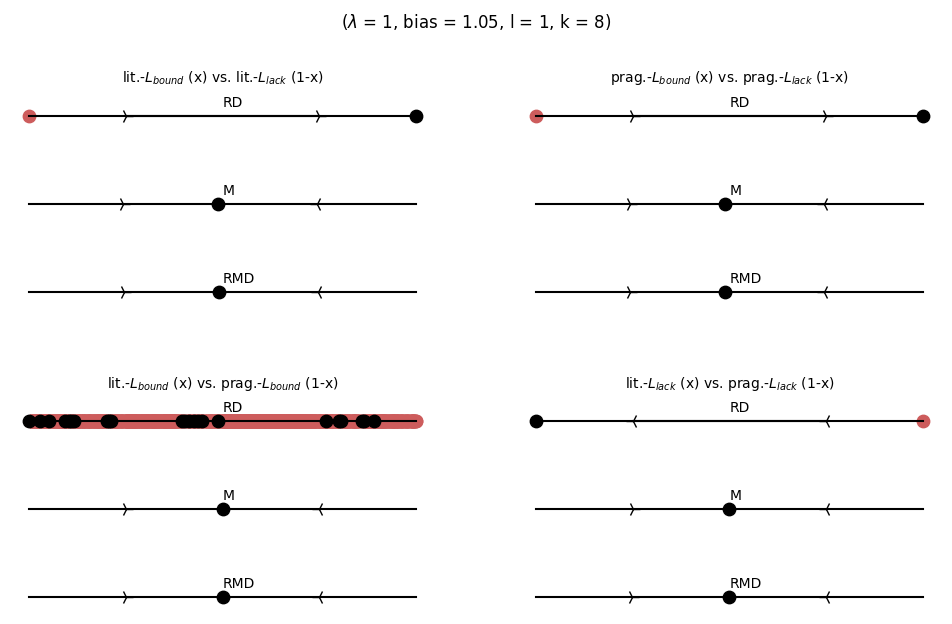
\includegraphics[scale=0.3]{phases-lam01-bias105-l01-k8}
  \caption{}
  \label{fig:sub1}
\end{subfigure}%
\begin{subfigure}{.6\textwidth}
  \centering
  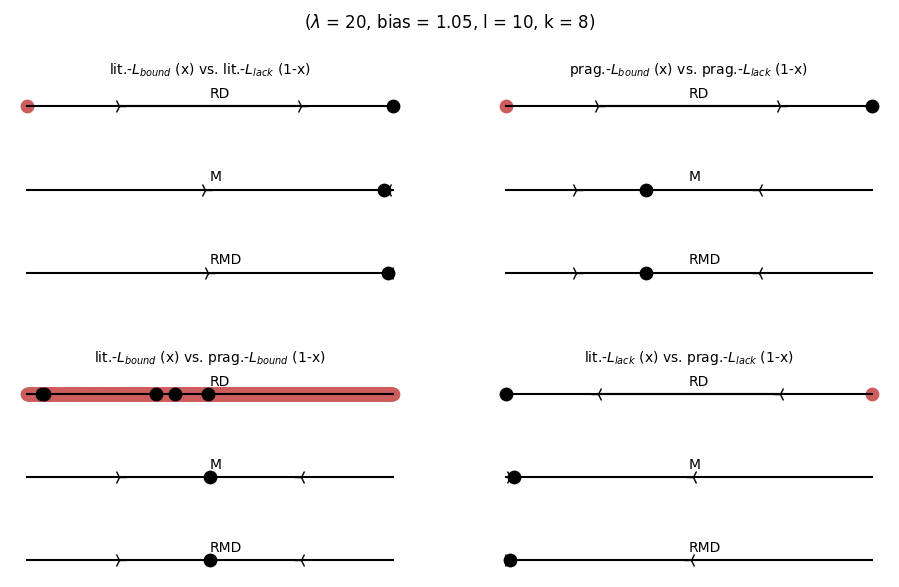
\includegraphics[scale=0.3]{phases-lam20-bias105-l10-k8}
  \caption{}
  \label{fig:sub2}
\end{subfigure}
\caption{Approximate phase-portraits for (a) $\lambda = 1, c = 1.05, l = 1, k = 8$ and (b) $\lambda = 20, c = 1.05, l =10, k =8$. Attractors are in black. Non-attractor points are in red for better visibility for lit. $\Lbound$ vs prag. $\Lbound$, which has many.}
\label{fig:phase}
\end{figure}


As before, Figure \ref{fig:phase} shows $8$ (approximate) portraits for applications of replicator steps only, mutator steps only, and replicator-mutator steps on our four type-pairings, for two parameter constellations ($c$ is now $1.05$ instead of $2$). For instance, the upper-left-most portrait shows the dynamic for a type space consisting of literal $\Lbound$ ($x$) and literal $\Llack$ ($1-x$). We can see that, as long as there are some $\Lbound$ types in the population, the population progresses toward the extreme where only this type survives. 

Beyond having cleaner portraits, my take on these is as before: They are nice because it's easy to see how the dynamics play out but they do not highlight difference between $M(x)$ and $M(RD(x))$ very well. The most pronounced differences I have found are when $\lambda$ is high, $c$ low, and learners tend to sample from the posterior posterior sampling (e.g.; $\lambda = 20$, $c = 1.05$, $l = 1$). However, that's a rather esoteric parameter constellation to illustrate the dynamics with. 


\subsection*{Dynamics}
\begin{figure}
\centering
\begin{subfigure}{.6\textwidth}
  \centering
  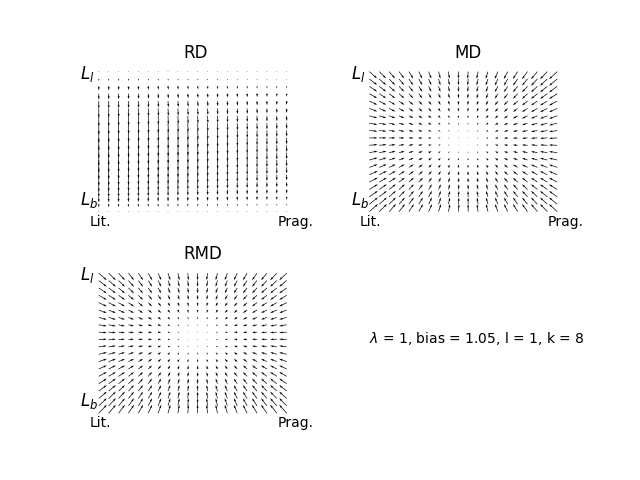
\includegraphics[scale=0.4]{quiver-lam1-c105-k8-l1}
  \caption{}
  \label{fig:sub1}
\end{subfigure}%
\begin{subfigure}{.6\textwidth}
  \centering
  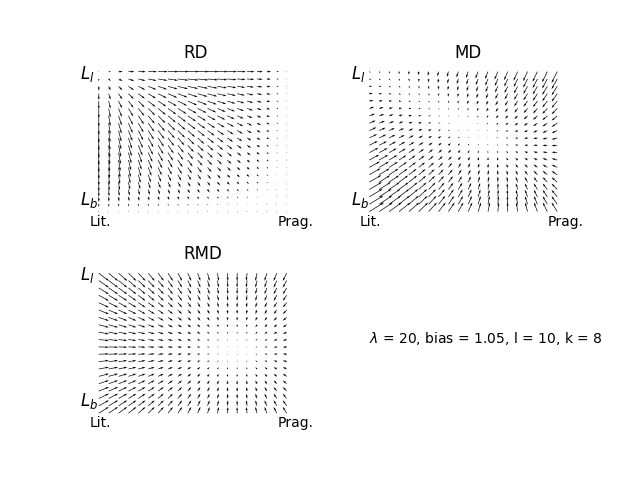
\includegraphics[scale=0.4]{quiver-lam20-c105-k8-l10}
  \caption{}
  \label{fig:sub2}
\end{subfigure}
\caption{Evolutionary competition between pairs of types with (a) $\lambda = 1, c = 1.05, l = 1, k = 8$ and (b) $\lambda = 20, c = 1.05, l =10, k =8$. Coordinates $(x,y)$ show (proportion of pragmatic types, proportion of $\Llack$ types).}
\label{fig:quivera}
\end{figure}


\begin{figure}
\centering
\begin{subfigure}{.6\textwidth}
  \centering
  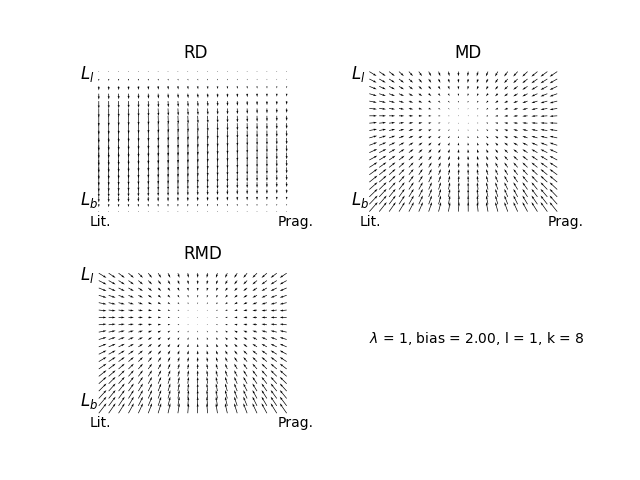
\includegraphics[scale=0.4]{quiver-lam1-c200-k8-l1}
  \caption{}
  \label{fig:sub1b}
\end{subfigure}%
\begin{subfigure}{.6\textwidth}
  \centering
  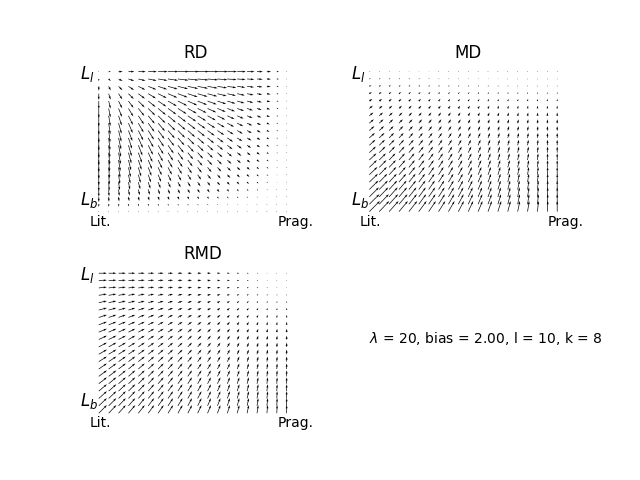
\includegraphics[scale=0.4]{quiver-lam20-c200-k8-l10}
  \caption{}
  \label{fig:sub2b}
\end{subfigure}
\caption{Evolutionary competition between pairs of types with (a) $\lambda = 1, c = 2, l = 1, k = 8$ and (b) $\lambda = 20, c = 2, l =10, k =8$. Coordinates $(x,y)$ show (proportion of pragmatic types, proportion of $\Llack$ types).}
\label{fig:quiverb}
\end{figure}

Figure \ref{fig:quivera} ($c = 1.05$) and Figure \ref{fig:quiverb} ($c = 2$) illustrate the new filled unit squares. The main news are that we got rid of the ambiguity for $(x,y)$ when we move away from the edges (see above). Taking stock: the good is that (i) the contrast between RD, M, and RMD is clear, (ii) we can see that lit. $\Llack$ is functionally disadvantageous and that its pragmatic counterpart is so as well if $\lambda$ is low, (iii) that a functional advantage {\em and} a learnability advantage will select for pragmatic $\Llack$ but not one of these on its own. The bad is that we don't see the slight functional disadvantage that prag. $\Lbound$ suffers from when compared to its literal counterpart.  



\end{document}
